\documentclass{article}
\usepackage[utf8]{inputenc}
\usepackage{hyperref}
\usepackage{graphicx}
\usepackage{float}
\usepackage[skip=10pt, indent=20pt]{parskip}
\graphicspath{{./figures/}{./lessons/03-lcd/assets/docs/figures/}}

\title{Lesson 23 - The LCD Display}
\author{Bryan A. \textit{CrazyUncleBurton} Thompson \\ \textit{bryan@batee.com}}
\date{March 11, 2026}

\begin{document}

\maketitle

\section*{Overview}

This lesson will introduce outputting to the LCD display.

\section*{Theory}
There is a lot to learn in the LCD lesson, so we will keep the circuit 
construction to a minimum.

\section*{Hardware Required}

The following hardware is needed for this lesson:

1 - M5Stack Tab5 Microcontroller Development Board

1 - M5Stack Dual Button Module

1 - 4 wire M5Stack sensor cable (comes with the Dual Button Module)

1 - USB cable to connect the Tab5 USB-C port to your PC
\vspace{30mm}


\section*{Objectives}

\begin{itemize}
  \item Draw static Text to the LCD using M5Unified.
  \item Draw static graphics to the LCD using M5GFX.
  \item Draw changing data to the LCD using M5Canvas.
  \item Build our Second Circuit.
  \item Build, Compile and Test the Programs.
  \item Note the differences in how data is displayed via various display 
  modes.
\end{itemize}
\vspace{2mm}


\section*{The Tab5 LCD Display}

This is a 5" 1280x720 (720P) IPS Touchscreen display with an ST7123 Display 
Driver Chipset.

There are many ways that we can write to this display:
\begin{itemize}
  \item M5Unified - This is a supplied text library from M5Stack.  It is quick
  to learn, and is best at displaying static data to the LCD.  If the data 
  changes over time, this will result in flickering screens.
  \item M5GFX - This is a supplied graphics library from M5Stack.  It is best 
  at displaying static Text and graphics to the LCD.  If the data changes 
  content or position over time, this will result in flickering screens.
  \item M5Canvas - This is an extension of M5GFX which treats 
  the screen as a framebuffer or canvas or sprite.  We draw the next screen to 
  a temporary "canvas" or sprite in the background.  When the next screen has 
  been updated, we push the canvas to the display.  The result is changes
  without the flicker-free nature of the previous libraries.
  \item LVGL / Squareline Studio.  LVGL is a non-factory library, and 
  Squareline Studio is an app that lets us create GUIs.  We will present this 
  in the later GUI lesson.

\end{itemize}
\vspace{2mm}


\section*{Connections}
\vspace{2mm}

\section*{The Program}
\vspace{2mm}


\section*{Compiling and Uploading the Program}

The microcontroller has \textit{bootloader} code running, which 
helps VS Code to upload programs to the microcontroller.  This code is preloaded
on the Tab5 at the factory, and remains in place when programs are uploaded to 
the microcontroller.

\begin{enumerate}
    \item See the upload port icon at the bottom of the screen. Ensure the upload 
    port is set to Auto. 
    \vspace{2mm}
    \begin{figure}[H]
        \centering
        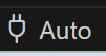
\includegraphics[width = .25\linewidth]{upload-port.png}
        \caption{PlatformIO: Upload Port}
    \end{figure}
    \vspace{2mm}
    \item To compile the program and upload it to the microcontroller, click 
    on the \textbf{PlatformIO: Build} icon at the bottom of the screen:
    \vspace{2mm}
    \begin{figure}[H]
        \centering
        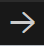
\includegraphics[width = .25\linewidth]{upload.png}
        \caption{PlatformIO: Upload}
    \end{figure}
    \vspace{2mm}
    \item Make sure the \textbf{Switch PlatformIO Project Environment} icon 
    at the bottom of the screen is set to \textbf{2-blink}.  This will ensure
    that we compile the correct code (there are many individual programs in
    the Microcontroller Training folder):
    \vspace{2mm}
    \begin{figure}[H]
        \centering
        
\includegraphics[width = .5\linewidth]{switch-platformio-project-environment.png}
        \caption{Switch PlatformIO Project Environment}
    \end{figure}
    \vspace{25mm}

    \item The results of the compile and upload process are presented in the 
    terminal window at the bottom of the screen:
    \vspace{2mm}
    \begin{figure}[H]
        \centering
        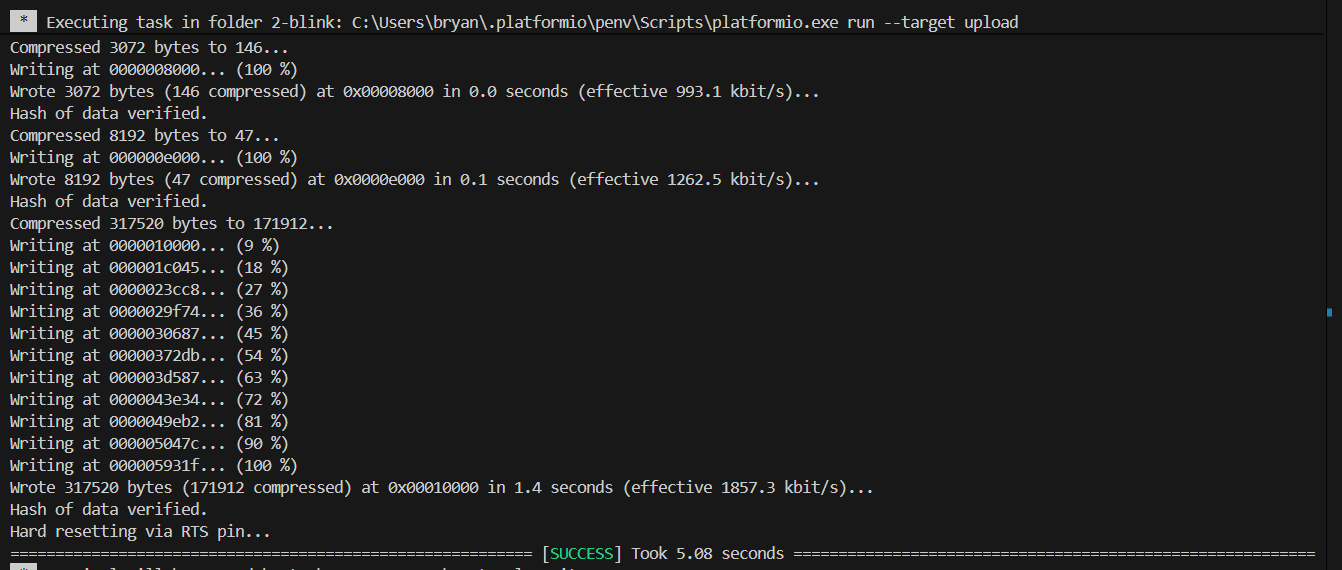
\includegraphics[width = 1\linewidth]{compiled.png}
        \caption{Program Compiled and Uploaded Successfully}
    \end{figure}
    \vspace{2mm}

\end{enumerate}

The compiled program is stored in FLASH memory on the microcontroller.  FLASH 
memory is persistent - it retains the program even after the power has been 
isconnected!

\vspace{2mm}
\section*{Running the Program}

When the program uploads and the microcontroller reboots, we should see the red 
and green LEDs alternating on and off every 1/2 second.


\vspace{2mm}
\section*{Conclusion}
This completes the the Getting Started / Hello World lesson.  In the next lesson, 
we will introduce the LCD screen.

\end{document}


